\documentclass[a4paper]{article}

\usepackage[T1]{fontenc}
\usepackage[utf8]{inputenc}
\usepackage[english]{babel}
\usepackage{csquotes}
\usepackage{listings}
\usepackage{multicol}
\lstset{language=c,frame=single,captionpos=b}
\usepackage{hyperref}
\usepackage{amsmath}
\usepackage[backend=biber, sorting=none,maxbibnames=40]{biblatex}
\renewbibmacro{in:}{}
\addbibresource{ref.bib}
\usepackage{graphicx}
\usepackage{placeins}
\usepackage[margin=2.5cm]{geometry}
\usepackage{subcaption}
\usepackage[affil-it]{authblk}
\usepackage{color}
\usepackage{amssymb,amsmath}
\usepackage{subfloat}
\usepackage{float}
\usepackage{framed}

\begin{document}
\title{JAVA Assignment: Rubik's Cube}
\author{Stefano Sandonà}
\affil{Vrije Universiteit Amsterdam, Holland}
\date{}
		
\maketitle

\section{The Rubik's Cube}
\label{sec:rubiks_cube}

A Rubik's Cube is a puzzle designed by Mr Rubik. In a Rubik's Cube, each of the faces is covered by colored stickers and in the initial setting, all the stickers of a face are of the same color and different colors are used for different faces. After performing some random twists, the goal of the game is to twist the cube until every side returns to be of a single color. 

\section{The Sequential Algorithm}
\label{sec:seq_algo}
The idea behind the sequential algorithm is simple. From a starting cube, we can twist it in each axis, row and direction (Figure \ref{fig:tw}) and from each cube of size \textit{S}, after a twist, there are \textit{6*(S-1)} new possible cubes. The evolution of the search can be represented as as a tree. 
The used state space search strategy, is the \textbf{deepening depth-first search (IDDFS)}. A depth-limited search is run repeatedly, increasing the depth limit with each iteration until it reaches d, the depth of the shallowest goal state. When the bound is increased, the solution search starts again from the begin (the root), and continues until the bound level is reached. On each iteration, the algorithm visits the nodes in the search tree in the same order as depth-first search, but the cumulative order in which nodes are first visited is effectively breadth-first. The first 2 iterations of the algorithm, with the order of the cube's evaluation is shown in Figure \ref{fig:iterations}. At the tree level \textit{i} there are \textit{(6*(S-1))\textsuperscript{i}} nodes (cubes), so there is a rapid growth of the search tree. The time complexity of IDDFS is O(b\textsuperscript{d}) and its space complexity is O(d), where b is the branching factor (\textit{6*(S-1)}) and \textit{d} is the depth of the shallowest goal.

\begin{figure}[ht]
  \centering
  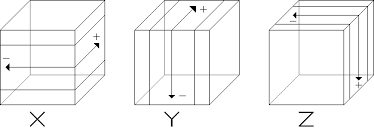
\includegraphics[width=0.5\linewidth]{xyz}
  \caption{Possible directions and axis for twists in a 3d cube}
  \label{fig:tw}
\end{figure}
\FloatBarrier

\begin{figure}
\begin{subfigure}{0.40\textwidth}
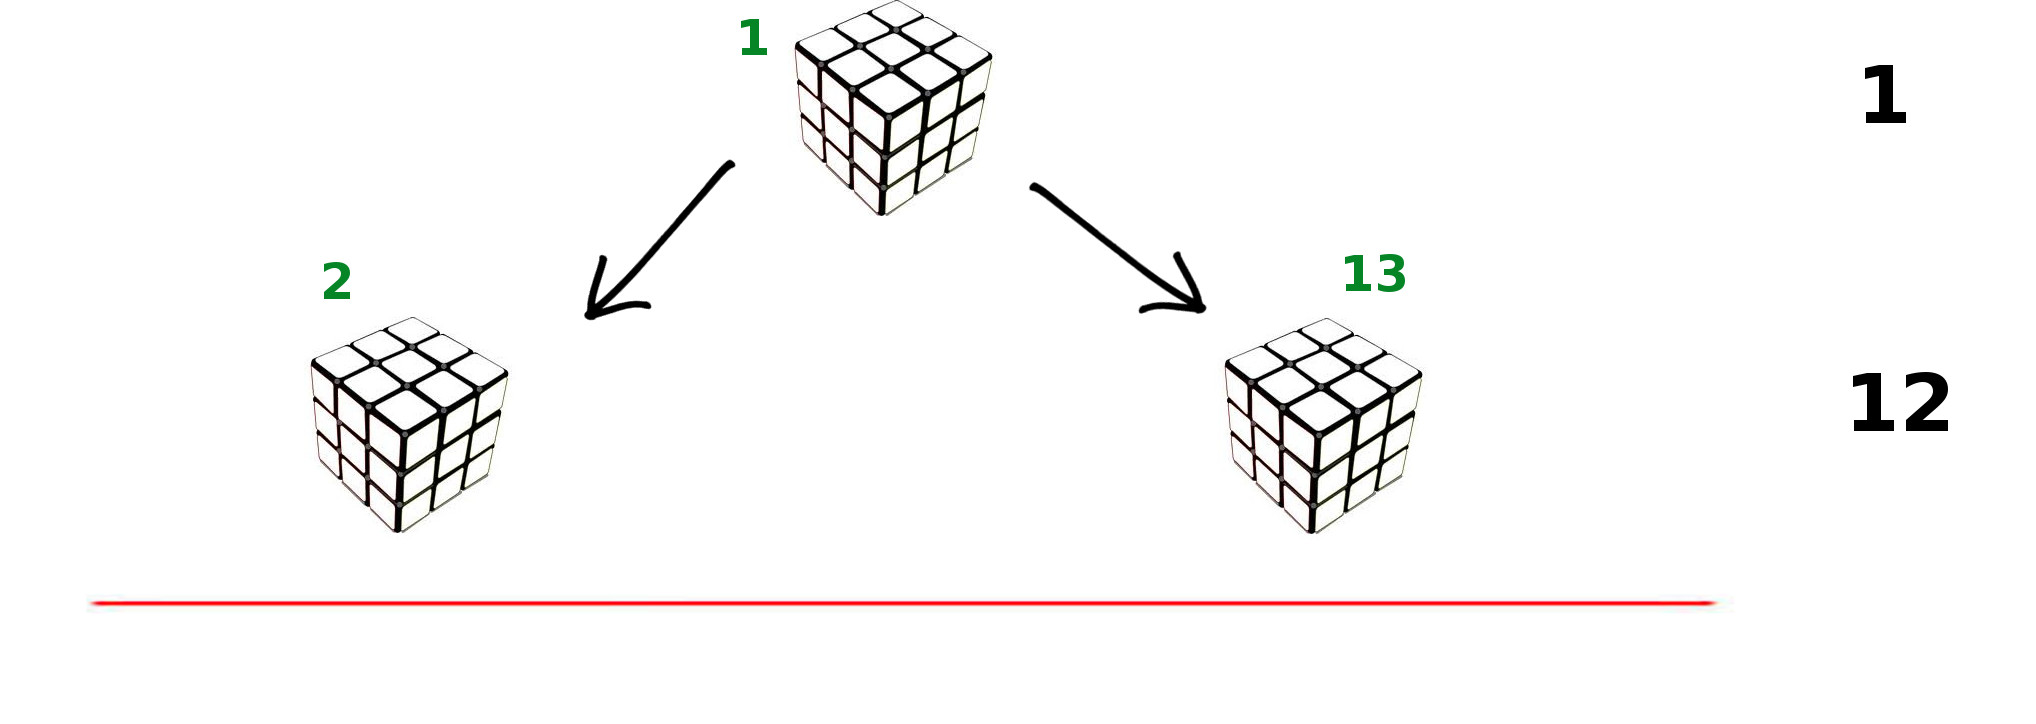
\includegraphics[width=\linewidth]{rubik_tree_eval1}
\caption{First itaration (bound=1)} \label{fig:ita}
\end{subfigure}
\hspace*{\fill} % separation between the subfigures
\begin{subfigure}{0.60\textwidth}
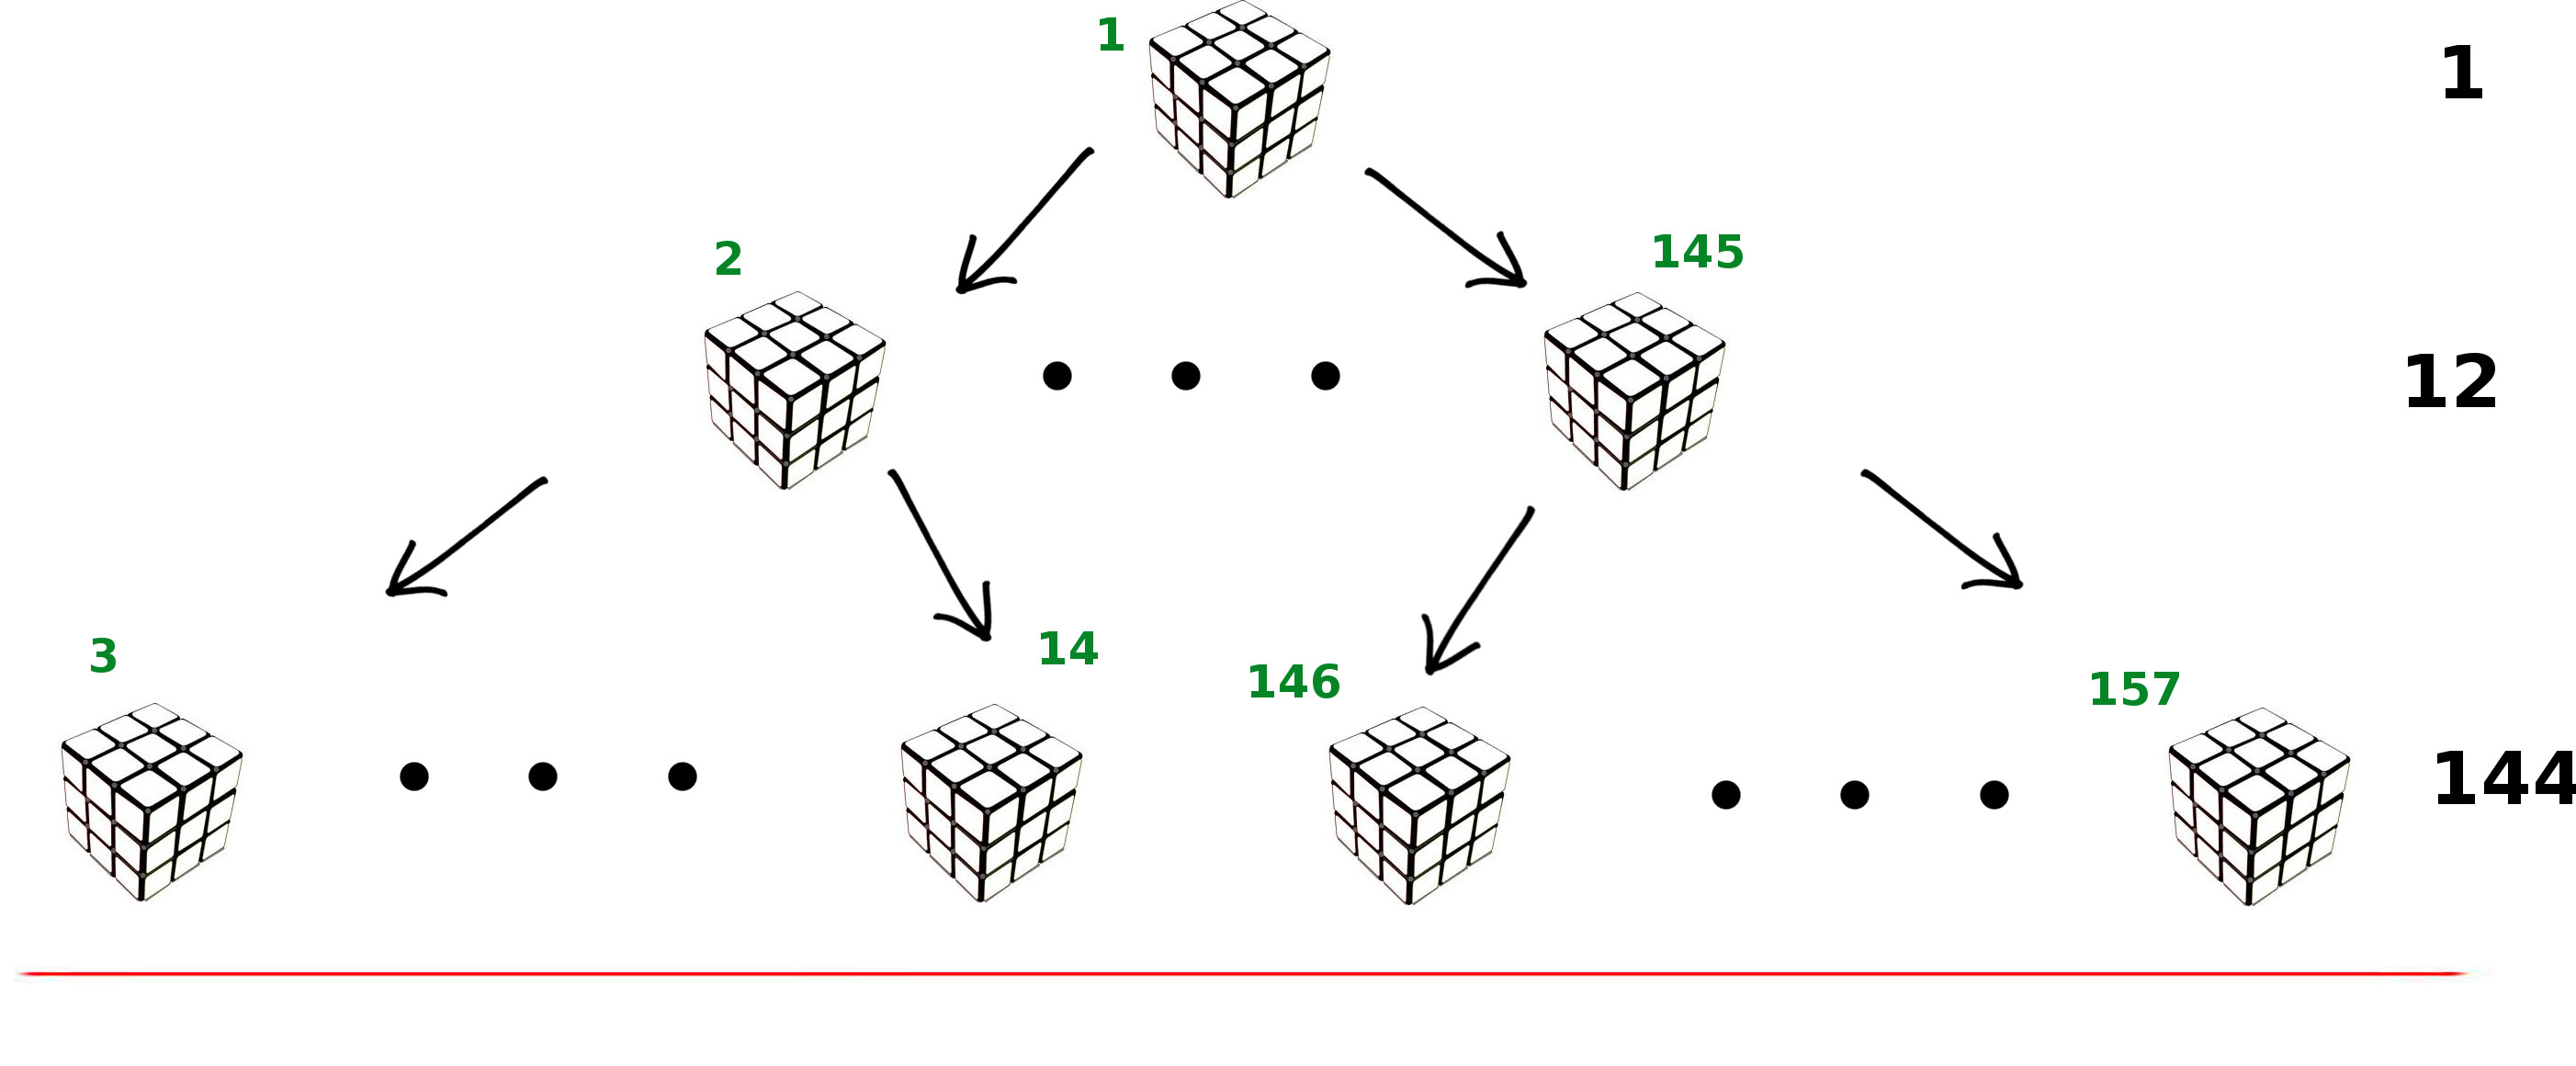
\includegraphics[width=\linewidth]{rubik_tree_eval2}
\caption{Second itaration (bound=2)} \label{fig:itb}
\end{subfigure}
\caption{The IDDFS Algorithm} \label{fig:iterations}
\end{figure}
\FloatBarrier

\section{The Parallel Algorithm}
\label{sec:par_algo}
An efficient parallelization of this algorithm is not trivial because of the work distribution. At each tree level, there are \textit{(6*(cubeSize-1))\textsuperscript{i}} cubes, and this number is most likely not a multiple of the available nodes involved in the computation. Another aspect, consist on the organization of the entire work, due to the fact that after a tree bound level is reached, the termination or the progress of the work has to be checked. The next paragraph was introduced to clarify terms and concepts that will be used in the rest of the report.

\subsection{The Ibis Portability Layer (IPL)}
\label{sec:ibis}
For this project was used an efficient platform for distributed computing: Ibis. This is a Java-centric communication system designed for grid computing, developed at VU University, Amsterdam. A fundamental concept in Ibis is the Pool, that is a set of one or more Ibis instances, often distributed in different machines. Each Ibis instance, that joined a specific pool, has an unique id and can cooperate with the others, running a single distributed application. With the election mechanism of Ibis, one machine can be elected as "master" and so be the "coordinator" or the central point of the entire work. Thanks to the registry mechanism, each Ibis instance can also know all the other Ibises that joined the same Pool and so communicate with them. The core of the Ibis system is the  Ibis Portability layer (IPL), that is a communication library specifically designed for usage in a grid environment. It is based on setting up connections. The programmer can create send/receive ports (with a name) and connect them in a flexible way: one-to-one, one-to-many, many-to-one. In addition, the programmer can define properties of connections and ports like reliability, FIFO ordering, ... . Proceeding in this way, after apply a certain configuration to a port, the only thing to do is to send a message through this port, the library will take care of the rest. 

\subsection{Cubes distribution}
\label{sec:cubes_distr}
The work distribution, or better the cubes distribution, is the central part of the parallel implementation. The more balanced is the work among the involved nodes and the more will be the achieved performance. The major problem with a static partitioning, is that at each tree level, a number multiple of 6 of cubes are generated, and this is often not perfect divisible by the number of involved machines. A naive approach could generate the first levels of the tree and when there are enough nodes (more than the number of Ibis instances involved), distribute them as fairly as possible. However, this could lead to a big load imbalance and, as conseguece, to have not good performance. For example, with a 3d cube and 5 machines, the tree will be unroll until level 1. The 12 resulting cubes would be divided into 3 3 2 2 2 and assigned to the 5 machines. This means that the first 2 machines would work 1.5 times the others. To outline the gravity of this, if \textit{m} (the tree level in which lives the solution) is big enough, it could be possible that the last 3 macchines worked for an entire day (24 hours), and the first two machines worked for one day and a half (36 hours). The total computational time would be 36 hours and for 12 hours the last 3 machines would be idle. 
The basic idea of amplify the tree until there are enough nodes is correct and logical, but the load imbalance factor must be considered. 

\subsubsection{Cube Weight}
\label{sec:cw}

To avoid the load imbalance, a way for measure the total amount of work assigned to a node is needed. To do this, to each cube could be assigned a "weight", based on the amount of the next cubes that will be generated from it. This weight is represented in Equation\ref{eq:eqWe}, where \textit{m} is the tree level in which there will be the solution(s) (unknown at the begin), \textit{n} is \textit{6*(cubeSize-1)} (the number of possible children per cube) and \textit{z} is the actual tree level of the cube.

\begin{equation} 
\label{eq:eqWe}
Weight = \sum_{i=0}^{m-z}{n^i}
\end{equation}
\FloatBarrier

As clarification, a practical example is reported in Figure \ref{fig:treeBin}. In this example, that is not related to the Rubik's Cube, but just to explain the general idea, \textit{n=2}, \textit{z1=1}, \textit{z2=2}, \textit{m=4}. Applying the previous formula, the weight of the first cube (at z1 level) is \textit{2\textsuperscript{0}+2\textsuperscript{1}+2\textsuperscript{2}+2\textsuperscript{3}=15}, because from it 14 cubes will be generated, so 15 (counting also the root node) will be evaluated in total. The weight of the second cube (at z2 level), is \textit{2\textsuperscript{0}+2\textsuperscript{1}+2\textsuperscript{2}=7}. 

\begin{figure}[ht]
  \centering
  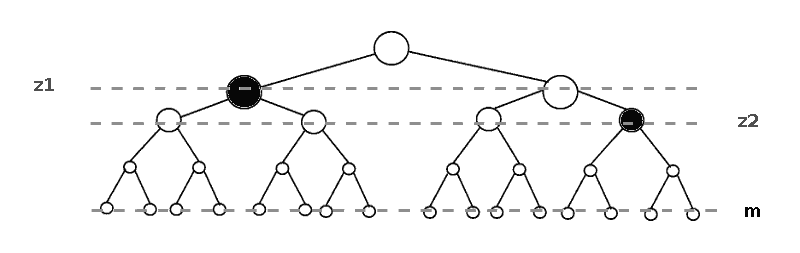
\includegraphics[width=0.8\linewidth]{tree_bin}
  \caption{Rubik's Cube Solution Tree}
  \label{fig:treeBin}
\end{figure}
\FloatBarrier

\subsubsection{Load balancing}
\label{sec:lb}

To have a fair ripartition of work. it is correct to assign to each Ibis instance more or less the same work to do. Given the fact that the number of cubes on a tree level often is not a multiple of the nodes involved on the computation, there will be load imbalance at a certain point. Also distributing the nodes at a specific tree level as fairly as possible, there will be one or more Ibis instances with one more cube than the others, for a gap of maximum one cube (e.g. with 9 cubes and 4 machines, 3 2 2 2). Accepting this, the best thing to do, is to select the correct tree level in which have this load imbalance, in order to limit the deriving damages. Looking at Equation\ref{eq:eqWe}, at the begin of the computation \textit{n} is known because it is the size of the cube, \textit{m} is unknown, is part of the solution, and \textit{z} is the value that we want to find. As just said, given enough cubes (more than the number of Ibis instances), the maximum difference of assigned cubes per node is one. This is possible using a simple \textit{for} construct (Listing \ref{fair}).

\begin{lstlisting}[label=fair, caption=fair distribution of cubes]
int sum = 0;
int rem = numCubes % numProcs; 
for (i = 0; i < numprocs; i++) {
    cubes_per_proc[i] = numCubes / numProcs;
    if (rem > 0) {
        cubes_per_proc[i]++;
        rem--;
    }
    displs[i] = sum;
    sum += cubes_per_proc[i];
}
\end{lstlisting}
\FloatBarrier

At a certain tree level \textit{z}, there are \textit{n\textsuperscript{z}} cubes and the relative weight per cube is the one shown in Equation\ref{eq:eqWe}. With the previous code (Listing \ref{fair}), calling \textit{k} the number of machines involved in the computation, the lowest amount of work assigned per slave, is shown in Equation \ref{eq:eqLow}, while the highest is shown in Equation \ref{eq:eqHig}. 

\begin{equation} 
\label{eq:eqLow}
LW=\sum_{i=0}^{m-z}{n^i}*\lfloor\frac{n^z}{k}\rfloor
\end{equation}
\FloatBarrier

\begin{equation} 
\label{eq:eqHig}
HW=\sum_{i=0}^{m-z}{n^i}*\lfloor\frac{n^z}{k}\rfloor +  \sum_{i=0}^{m-z}{n^i}
\end{equation}
\FloatBarrier

To reduce the load imbalance as much as possible, the two amounts of work should differ as little as possible. That means that \textit{HW*100/LW} has to be as near to 100 as possible, for example lower than 101, that means that a maximum of 1\% of load imbalance is permitted. Solving the inequality shown in Equation \ref{eq:eqIne}, the solution is the one shown in Equation \ref{eq:eqSol}. 

\begin{equation} 
\label{eq:eqIne}
\frac{(\sum_{i=0}^{m-z}{n^i}*\lfloor\frac{n^z}{k}\rfloor +  \sum_{i=0}^{m-z}{n^i})*100}{(\sum_{i=0}^{m-z}{n^i}*\lfloor\frac{n^z}{k}\rfloor)} < 101
\end{equation}
\FloatBarrier

\begin{equation} 
\label{eq:eqSol}
\lfloor\frac{n^z}{k}\rfloor > 100
\end{equation}
\FloatBarrier

At the begin \textit{n} (the size of the cube) is known and also \textit{k} (the number of Ibises that joined the pool), so the value to find is \textit{z}. In addition to reduce the load imbalance, it's useful to reduce the initial tree unroll at the minimum. For this reason, the final value to find is the one shown in Equation \ref{eq:eqSol2}.

\begin{equation} 
\label{eq:eqSol2}
\min_{z>0} \lfloor\frac{n^z}{k}\rfloor > 100
\end{equation}
\FloatBarrier

\subsubsection{Work split}
\label{sec:ws}

Once found the correct value of \textit{z}, this is the tree level in which to have an imbalance of 1 cube, isn't such a big risk for the performance. 
To reduce the unroll, the tree is extended (A) until the level \textit{z-1}, if at that level there are enough nodes (more than the Ibis instances), otherwise (B) until the level \textit{z}. If we are in case A, the \textit{n\textsuperscript{(z-1)}} resulting nodes are divided into equal parts to the machines (\textit{n\textsuperscript{(z-1)}/k} cubes per machine). If some nodes have left out (\textit{k} is not a divisor of the number of nodes of this level), these are expanded to the next tree level (Figure \ref{fig:ev1}), otherwise the splitting phase is terminated (Figure \ref{fig:ev2}). If we have expanded some nodes, we try to split their children among the Ibis instances. Until they are less than the number of ibis instances we generate another level of the tree from them (Figure \ref{fig:ev3}). When they are enough, we split them as fairly as possible (using the approach shown in Listing \ref{fair}). If we are in case B we just split the \textit{n\textsuperscript{(z)}} nodes as fairly as possible (Listing \ref{fair}). In Figure \ref{fig:ev1}, Table \ref{table:tev1} there is an example of work riparitition among 11 Ibis instances, in Figure \ref{fig:ev2}, Table \ref{table:tev2} among 16 Ibis instances and in Figure \ref{fig:ev3}, Table \ref{table:tev3} among 13 Ibis instances. 

\begin{figure}[!ht]
  \centering
  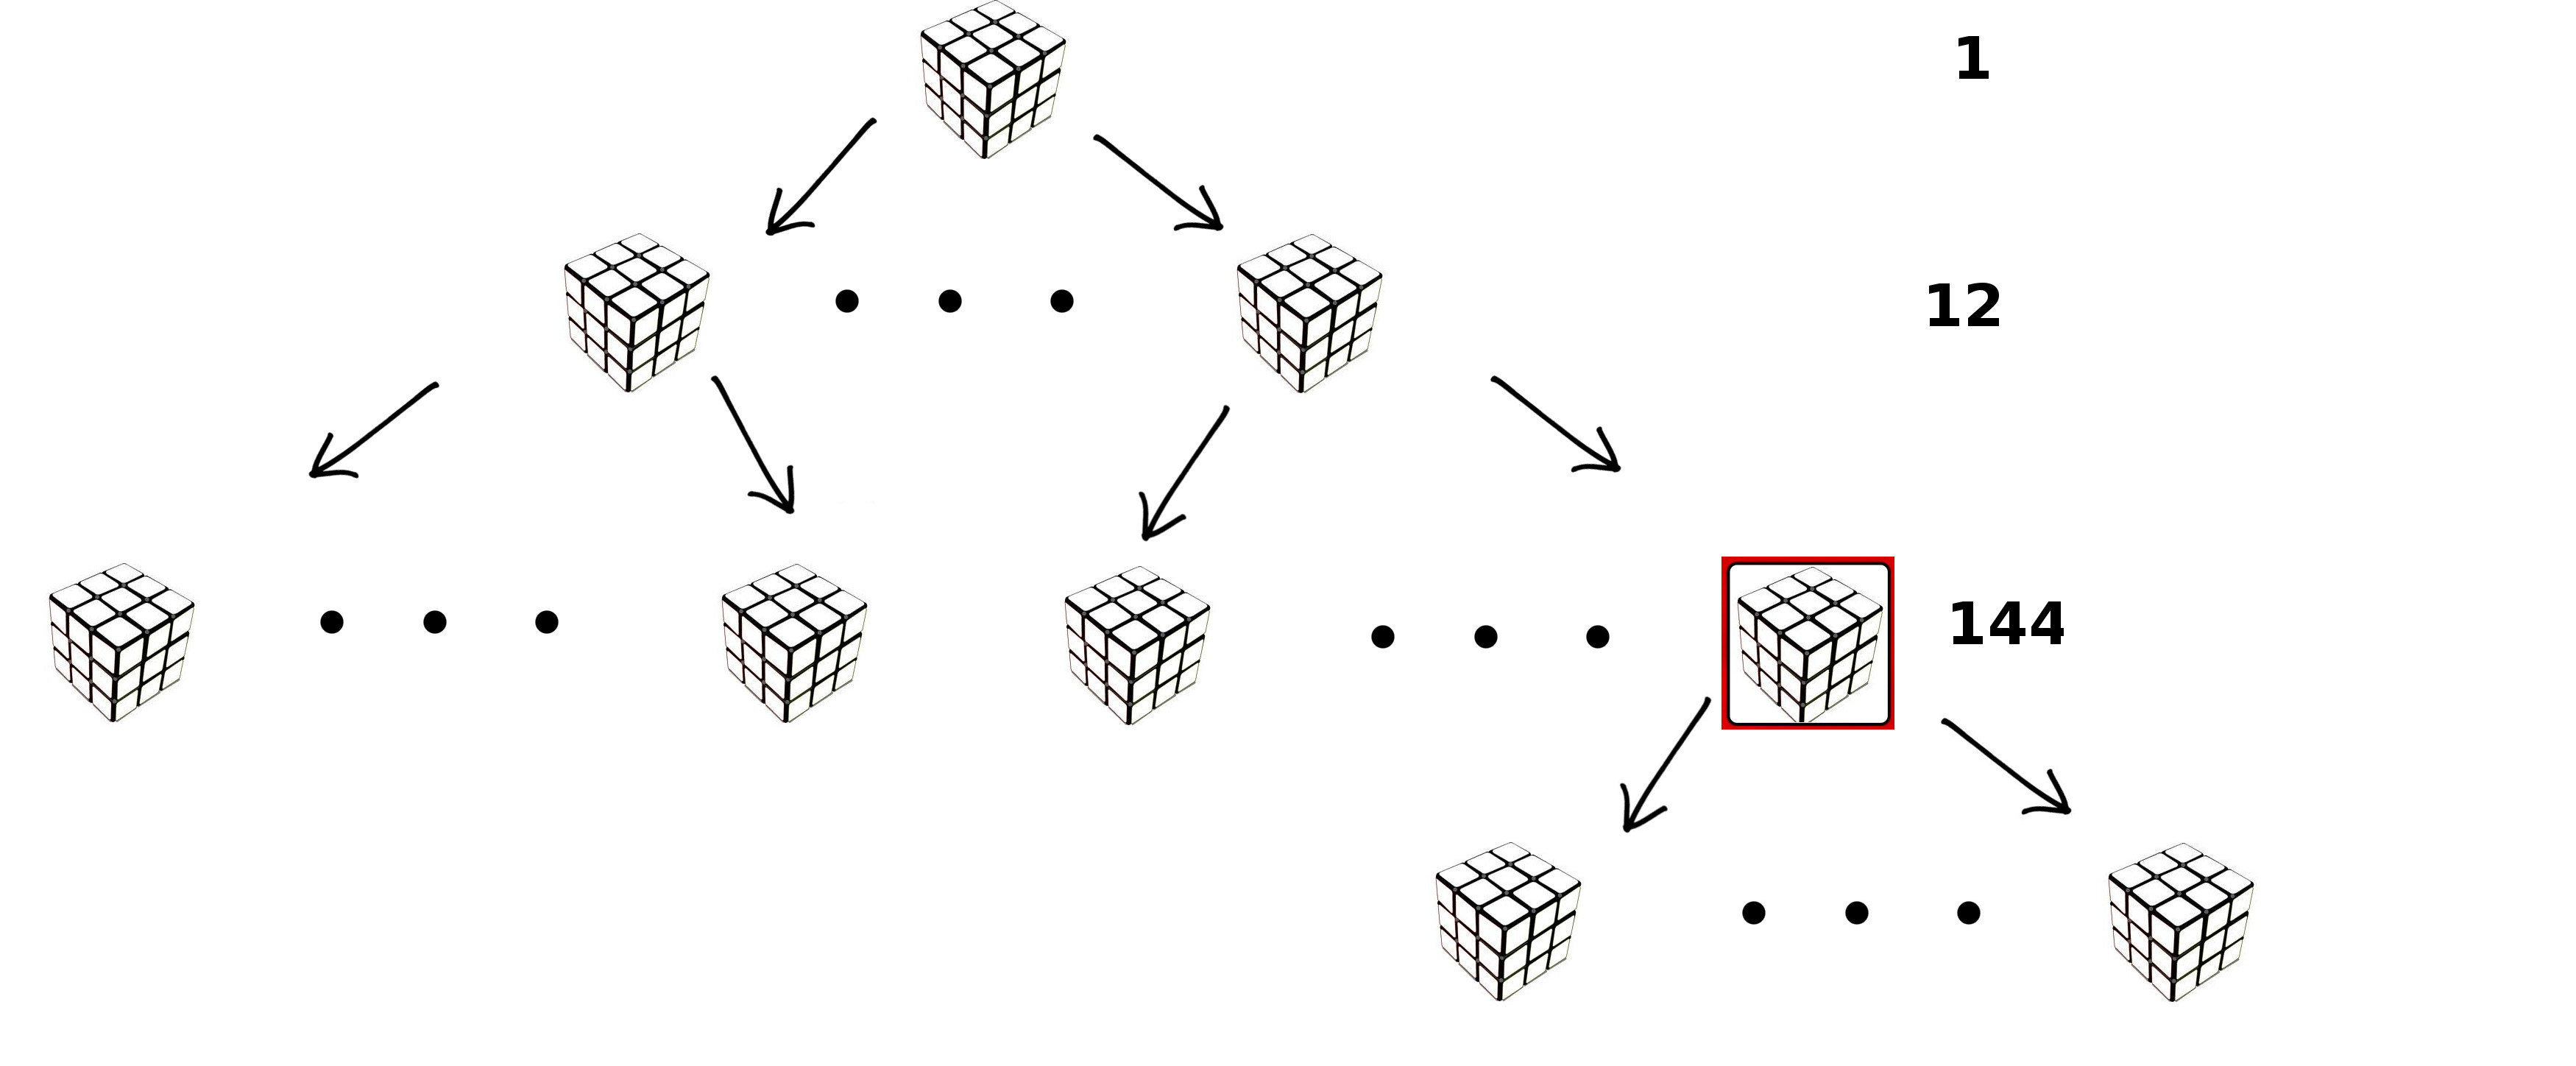
\includegraphics[width=0.7\linewidth]{rubik_tree_eval3}
  \caption{Cubes distribution - Ibis instances=11, Size=3, Twists=11, Bound=7}
  \label{fig:ev1}
\end{figure}
\FloatBarrier

\begin{table}[!ht]
\centering
\begin{tabular}{|l|l|l|l|l|l|l|l|l|l|l|l|l|l|l|}
\multicolumn{1}{|c||}{\bfseries Ibis Instance} & 0 & 1 & 2 & 3 & 4 & 5 & 6 & 7 & 8 & 9 & 10 & \multicolumn{1}{|c|}{\bfseries Total} \\ \hline
\multicolumn{1}{|c||}{\bfseries Cubes of level 2} & 13 & 13 & 13 & 13 & 13 & 13 & 13 & 13 & 13 & 13 & 13 & 143 \\ \hline
\multicolumn{1}{|c||}{\bfseries Cubes of level 3} & 2 & 1 & 1 & 1 & 1 & 1 & 1 & 1 & 1 & 1 & 1 & 12
\end{tabular}
\caption{Cubes distribution - Ibis instances=11, Size=3, Twists=11, Bound=7}
\label{table:tev1}
\end{table}
\FloatBarrier

\begin{figure}[!ht]
  \centering
  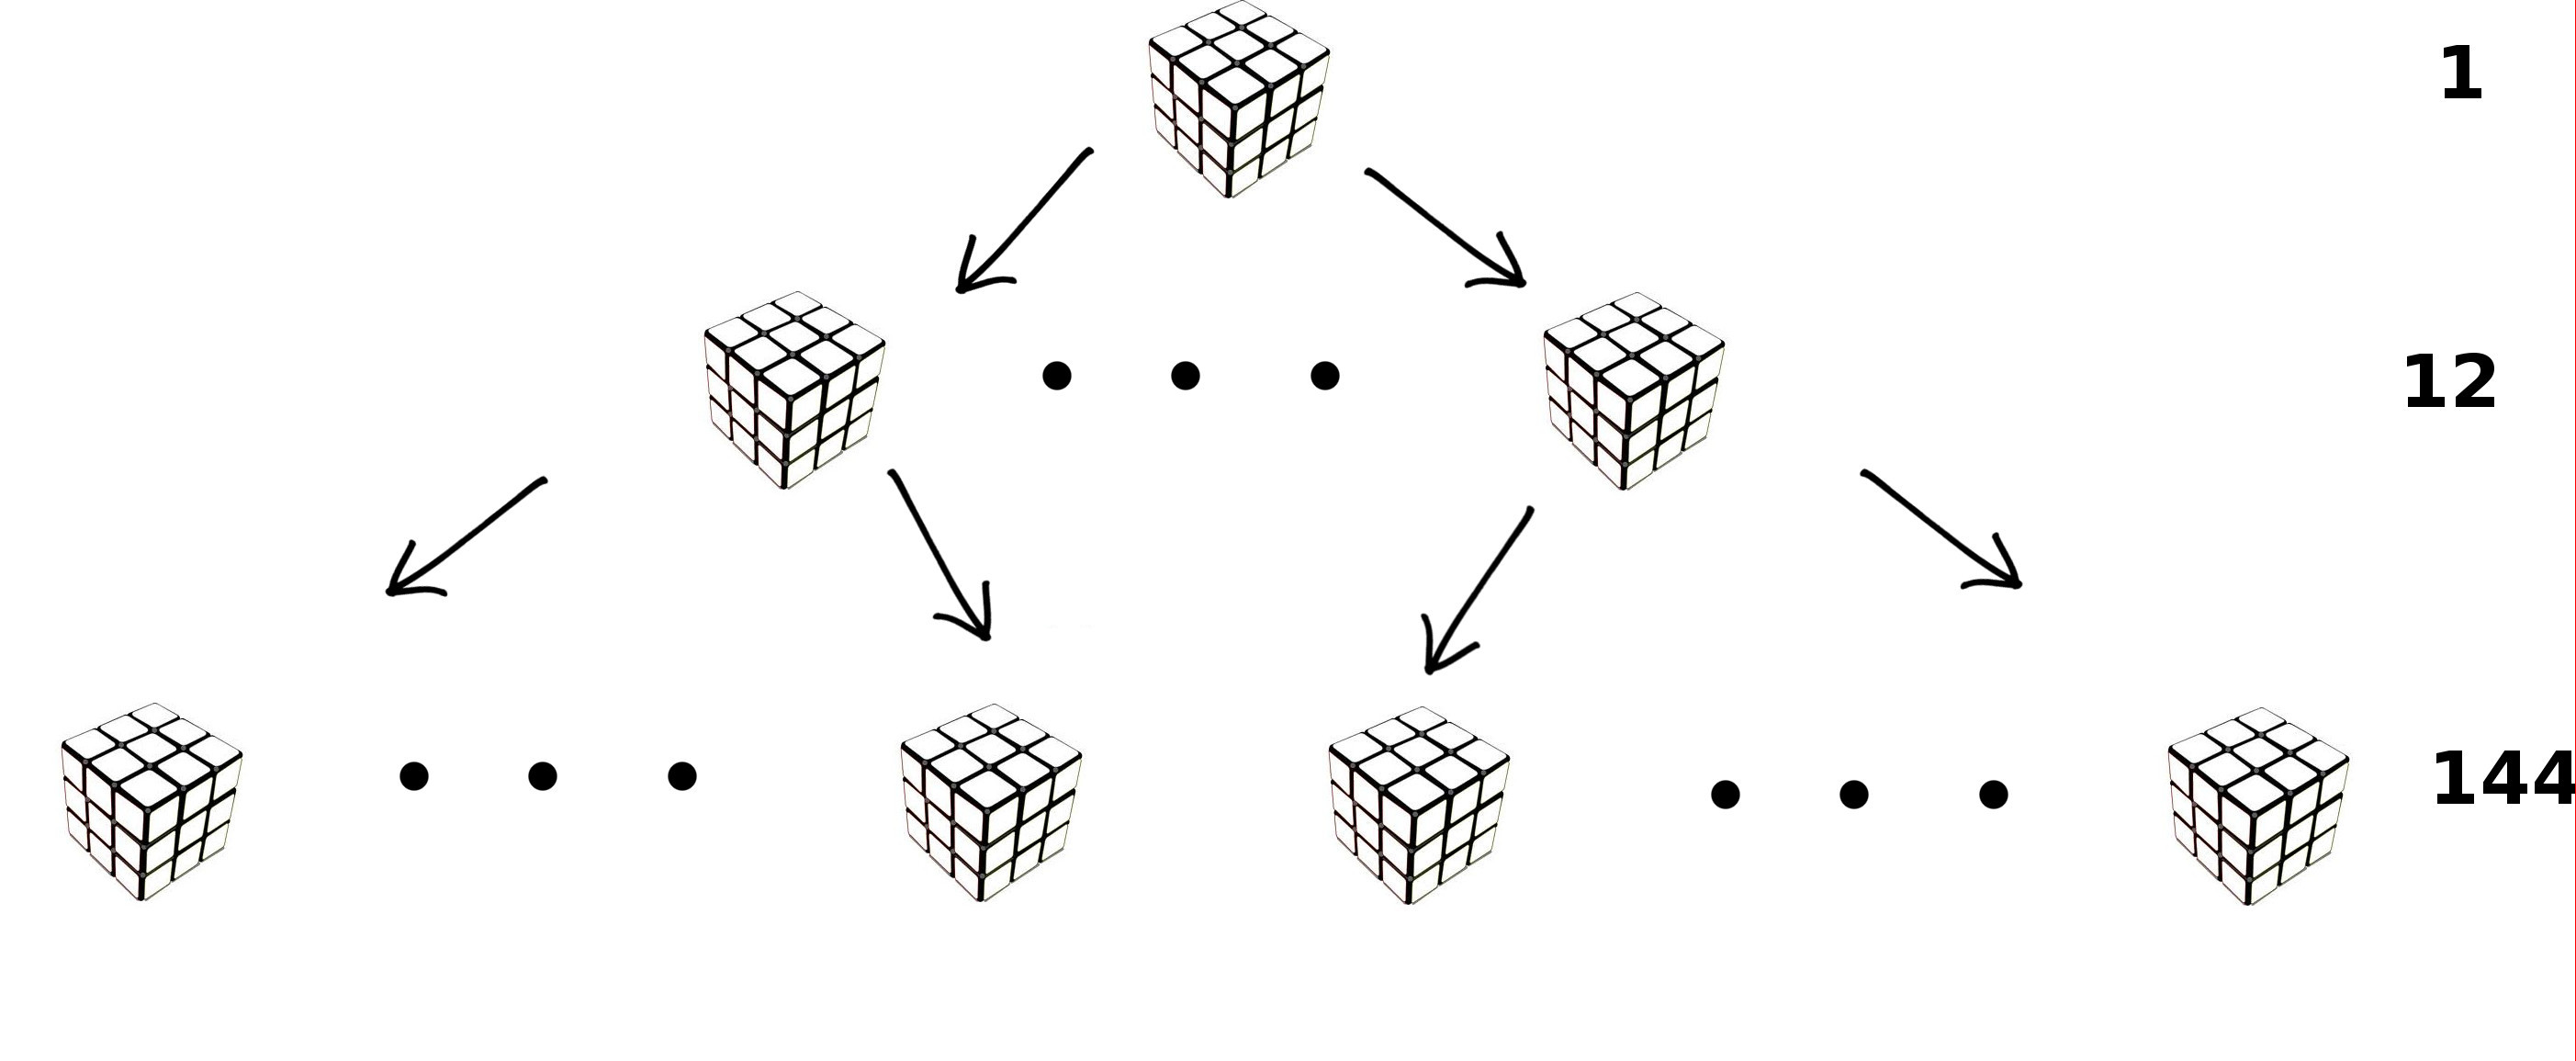
\includegraphics[width=0.7\linewidth]{rubik_tree_eval5}
  \caption{Cubes distribution - Ibis instances=16, Size=3, Twists=11, Bound=7}
  \label{fig:ev2}
\end{figure}
\FloatBarrier

\begin{table}[!ht]
\centering
\begin{tabular}{|l|l|l|l|l|l|l|l|l|l|l|l|l|l|l|l|l|l|}
\multicolumn{1}{|c||}{\bfseries Ibis Instance} & 0 & 1 & 2 & 3 & 4 & 5 & 6 & 7 & 8 & 9 & 10 & 11 & 12 & 13 & 14 & 15 & \multicolumn{1}{|c|}{\bfseries Total} \\ \hline
\multicolumn{1}{|c||}{\bfseries Cubes of level 2} & 14 & 14 & 14 & 14 & 14 & 14 & 14 & 14 & 14 & 14 & 14 & 14 & 14 & 14 & 14 & 14 & 144 
\end{tabular}
\caption{Cubes distribution - Ibis instances=16, Size=3, Twists=11, Bound=7}
\label{table:tev2}
\end{table}
\FloatBarrier

\begin{figure}[!ht]
  \centering
  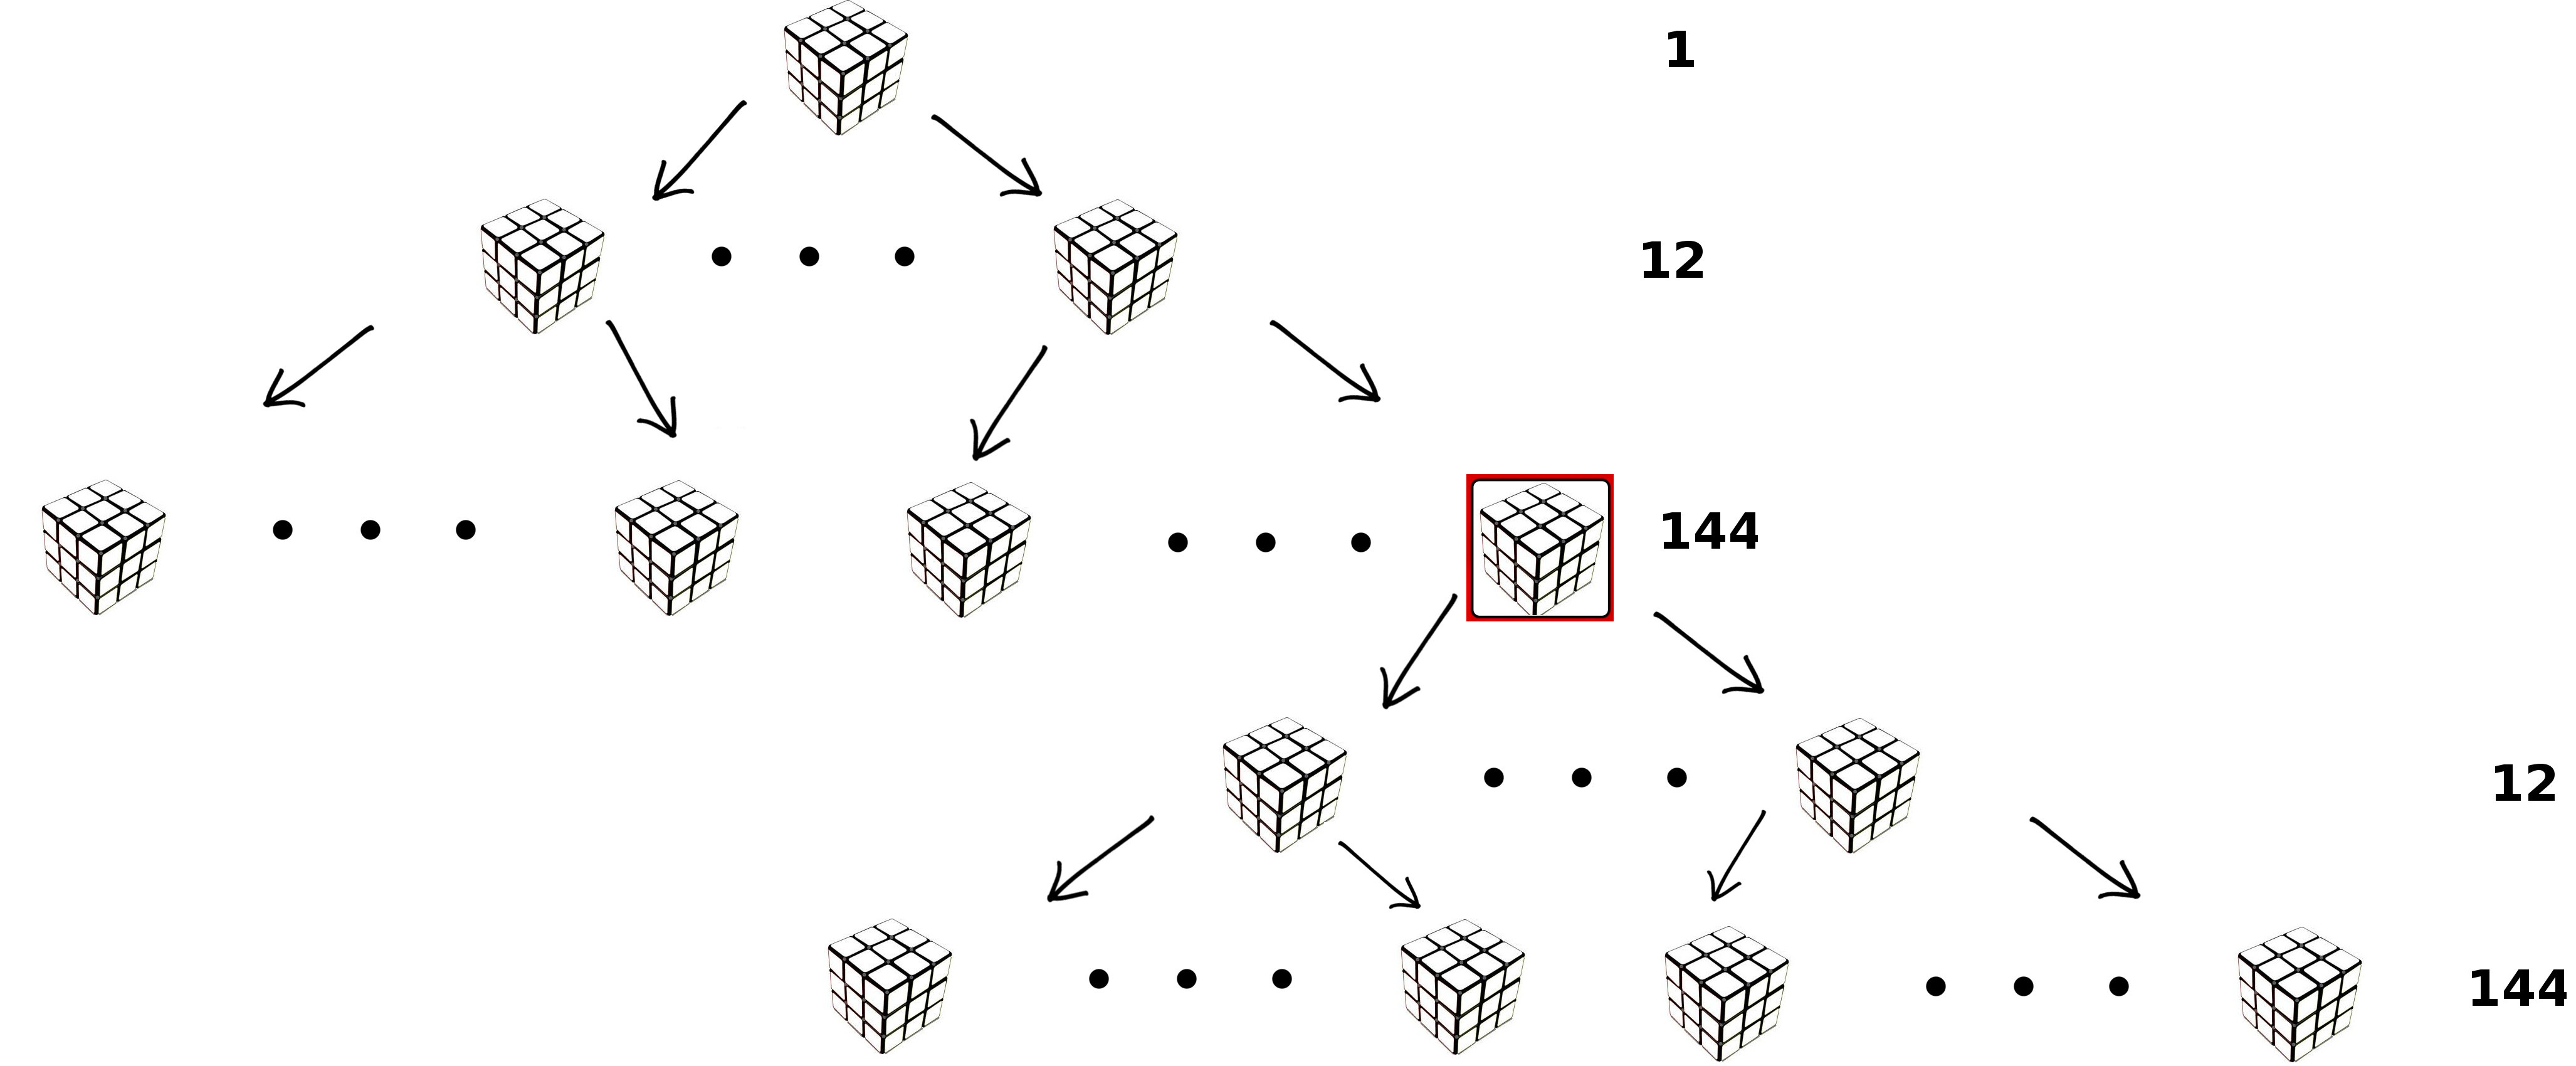
\includegraphics[width=0.7\linewidth]{rubik_tree_eval4}
  \caption{Cubes distribution - Ibis instances=13, Size=3, Twists=11, Bound=7}
  \label{fig:ev3}
\end{figure}
\FloatBarrier

\begin{table}[!ht]
\centering
\begin{tabular}{|l|l|l|l|l|l|l|l|l|l|l|l|l|l|l|}
\multicolumn{1}{|c||}{\bfseries Ibis Instance} & 0 & 1 & 2 & 3 & 4 & 5 & 6 & 7 & 8 & 9 & 10 & 11 & 12 & \multicolumn{1}{|c|}{\bfseries Total} \\ \hline
\multicolumn{1}{|c||}{\bfseries Cubes of level 2} & 11 & 11 & 11 & 11 & 11 & 11 & 11 & 11 & 11 & 11 & 11 & 11 & 11 & 143 \\ \hline
\multicolumn{1}{|c||}{\bfseries Cubes of level 3} & 0 & 0 & 0 & 0 & 0 & 0 & 0 & 0 & 0 & 0 & 0 & 0 & 0 & 0  \\ \hline
\multicolumn{1}{|c||}{\bfseries Cubes of level 4} & 12 & 11 & 11 & 11 & 11 & 11 & 11 & 11 & 11 & 11 & 11 & 11 & 11 & 144
\end{tabular}
\caption{Cubes distribution - Ibis instances=13, Size=3, Twists=11, Bound=7}
\label{table:tev3}
\end{table}
\FloatBarrier

In Table \ref{table:tlow}, are reported the numbers of cubes evaluated by each Ibis instance, when the algorithm's bound is 7, with a Cube of size 3. These numbers were measured running the implementation with different number of Ibises. The Expanded Cubes, are the ones from which are generated other cubes during the initial splitting work phase while the Assigned Cubes are the ones effectively evaluated. As shown, for every launching configuration, the load imbalance is always under the 1\%.

\centering
\begin{table}[!ht]
\centering
\caption{Cubes distribution - Size=3, Twists=11, Bound=7}
\label{table:tlow}
\begin{tabular}{l|l|l|l|l}
\multicolumn{1}{c}{\bfseries Ibis Instance} & \multicolumn{1}{c}{\bfseries Assigned Cubes} & \multicolumn{1}{c}{\bfseries Expanded Cubes} & \multicolumn{1}{c}{\bfseries Total Cubes} & \multicolumn{1}{c}{\bfseries Load Imbalance} \\ \hline
2 & 19544622 & 1 & 39089245 & 0\%  \\ \hline
4 & 9772311 & 1 & 39089245 & 0\% \\ \hline
5 & 7804273(2), 7826894(3) & 17 & 39089245 & 0,28\% \\ \hline
8 & 4886154 & 13 & 39089245 & 0\% \\ \hline
11 & 3551510(10), 3574131(1) & 14 & 39089245 & 0.63\% \\ \hline
13 & 3006718(12), 3008603(1) & 26 & 39089245 & 0.06\%
\end{tabular}
\end{table}
\FloatBarrier

\subsection{Solution search and Ibises coordination}
\label{sec:ibis_setting}
After the cubes of the first levels are correclty splitted, each Ibis instance will have a work queue and for each cubes inside it, the algorithm will proceed like in the sequential version. To avoid the initial send of the cubes, each Ibis instance will generate the same initial cube, will perform the splitting phase and will assign certain cubes to itself. To reach the final solution, the machines involved in the computation have to coordinate and cooperate. When a tree level bound is reached, the distributed results have to be summed, in order to decide if continue with the next bound or not. To do that, a "master slave" approach s adopted. The "master" Ibis instance collects and sums the partial results and decides if the work is finished or continue with the next bound. For what concerning the communication setting, 4 ports are used. On the master side 2 ports are needed, one to receive the results from the slaves and one to communicate them if the  the work is finisched. Specularly, on the slaves side, 2 ports are needed, one to communicate the solution found and one to receive if the next bound has to be evaluated or the work is finished. A graphic representation of the ports organization is presented in Figure \ref{fig:ports}.

\begin{figure}
\begin{subfigure}{0.5\textwidth}
\centering
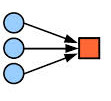
\includegraphics[width=0.5\linewidth]{results}
\caption{Results communication - Many to 1} \label{fig:ca}
\end{subfigure}
\hspace*{\fill} % separation between the subfigures
\begin{subfigure}{0.5\textwidth}
\centering
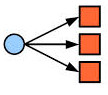
\includegraphics[width=0.5\linewidth]{continue}
\caption{Work status communication - 1 to Many} \label{fig:cb}
\end{subfigure}
\caption{Send (circle) and Receive (square) Ports organization} \label{fig:ports}
\end{figure}
\FloatBarrier

\subsubsection{Special cases}
\label{sec:sc}
The worst part of this implementation, is that it performs the tree unrolling phase at the begin of each bound increase, in order to better distribute the work. During this step, it's possible to find the problem solution if the cube was previously twisted for few times. However, that would means a small searching space, and so a non convenience on solving the cube in parallel. In the case a tree level is completely generated during the initial unrolling phase and a solution is found, the current algorithm will stops, and the master Ibis will show the problem solution, without performing any extra communication with the slaves. Another border case, is that we are unlucky and performing the second tree extension with the cubes left out by the division (in the Figure \ref{fig:ev1} the cube surrounded by the red square), these are solved cubes. The algorithm, correctly treat also this scenario, storing the partial results found at each level of the unrolling and adding these to the tree level results found during the next solving phase.

\subsection{Results}
\label{sec:results}


\printbibliography 

\end{document}